\begin{Exercise}[title=Cartouche pour vélo]
  \begin{minipage}{0.7\linewidth}
    On considère une cartouche  contenant $16 g$ de $CO_2$.\\
    \emph{Dimension}: \\
    Diamètre: 2,2 cm \\
    Diamètre au goulot: 9,2 mm en haut du filetage \\
    Longueur de la cartouche: 8,84 cm \\
    \emph{Donnée}:
    $P_{sat}(CO_{2},298K) = 5MPa$
    
  \end{minipage}\hspace{.05\linewidth}
  \begin{minipage}{0.2\textwidth}
    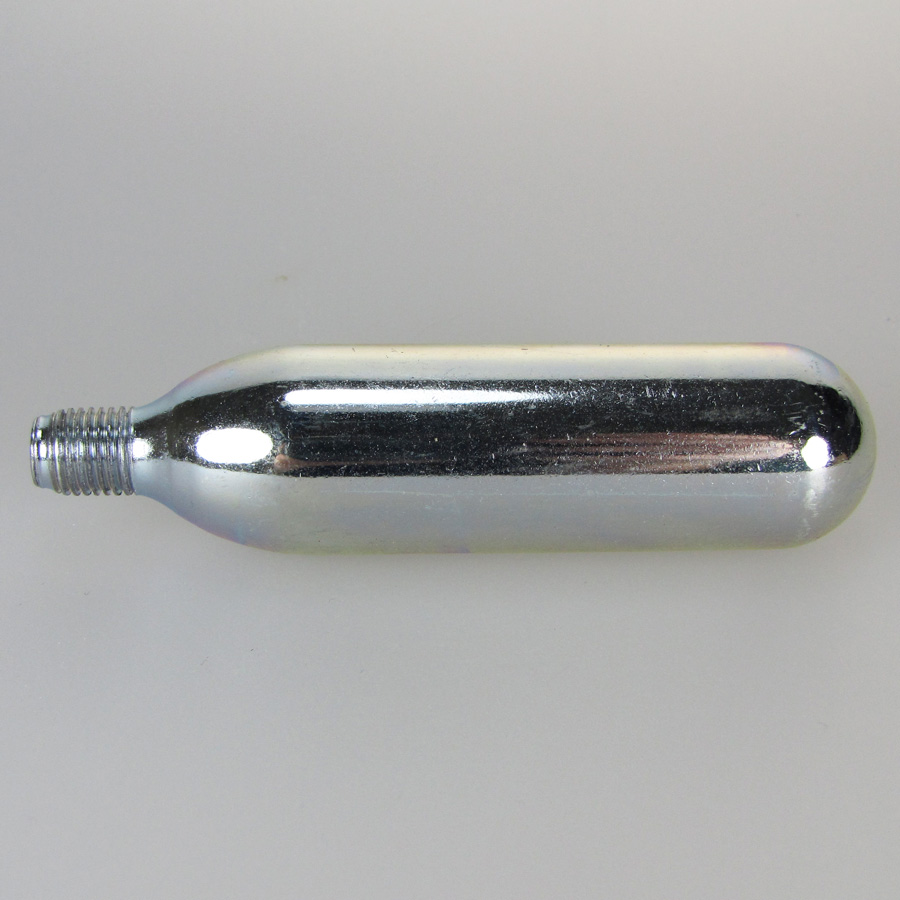
\includegraphics[width=\linewidth]{../fig/cartouche.jpg}
  \end{minipage}

  Lorsque qu'on décharge la capsule, sa surface gèle.
  \Question Quelle est la composition de la cartouche de gaz
  \Question Peut on gonfler une roue de vélo avec une telle cartouche, proposez des valeurs numérique?
\end{Exercise}
\begin{Answer}
		On a Le volume de la cartouche $V_c= 33,6.10^{-6}$  et \gdr{rho_l}{1032}{\kg\per\m\cubed}.Sur le diagramme d'état on relève $P_{sat} = 5 $MPa à 298K. Si le $CO_2$ est seulement gazeux, on a:
		\[ P_{CO_2} = \frac{mRT}{\mathcal{M}_{CO_2}V_c} \geq P_{sat} \]
		Une partie du gaz est sous forme liquide (comme dans les bombone de gaz classique).
		\emph{vous pouvez donner la composition du mélange ?}
		\[
		\begin{cases}
		P_{sat} V_g &= n_g R T \\
		V_l &= \frac{n_l \mathcal{M}}{\rho_l} \\
		(3)~~ V_l +V_g &=V_c \\
		n_l +n_g &= n
		\end{cases}\]
		On prend une chambre à air avec un rayon de 60cm et une section de rayon 2cm, on la veux gonfler entre 2 et 4 bars. Avec la loi des gaz parfait on a
		\[P_{roue} =    \frac{mRT}{\mathcal{M}_{CO_2}V_{roue}} \sim 3 bar \]
		Normal on les vends à Décathlon.
\end{Answer}
